% ----------------------------------------------------------
\chapter{Estruturas de busca de pontos}\label{cap:desenvolvimento}
% ----------------------------------------------------------
Neste capitulo apresentamos uma visão de como funcionam as consultas de objetos geométricos. 
São os algoritmos e estruturas de dados base para a construção de um controle de janela para acesso rápido de polígonos
em um mundo e queremos saber quais polígonos estão na consulta.

% ----------------------------------------------------------
\section{Árvore KD}
% ----------------------------------------------------------

Árvore KD é uma árvore binaria onde cada folha é um ponto \textit{k-dimensional}.
Cada nó não-folha é um corte em uma dimensão, representando implicitamente um hiperplano.
Pontos à esquerda desse hiperplano estão na subárvore da esquerda, e respectivamente para o lado direito.
Cada nó é associado com uma das \textit{k dimensões}. Então, a citar um exemplo, se dado nó divide o eixo
x, a subárvore a esquerda contem os pontos com o eixo x menor que o ponto de corte.

\begin{figure}[htb]
    \caption{\label{fig:Fig_1}Árvore \textit{3-dimensional}}
    \begin{center}
        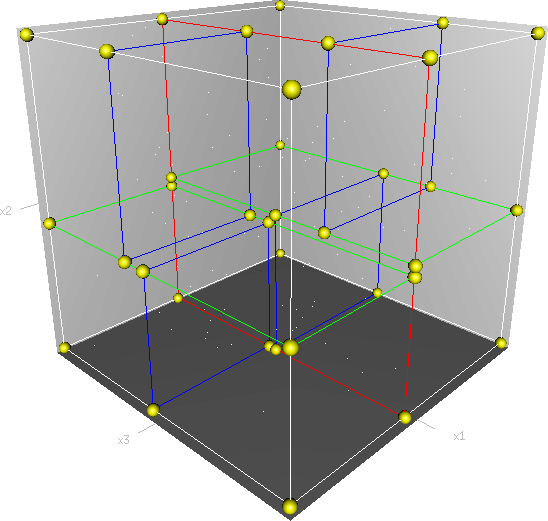
\includegraphics[width=\linewidth/2]{./images/3dtree.png}
    \end{center}
    \fonte{GPL}
\end{figure}

\subsection{Arvore 2D}
Arvore 2-dimensional é a implementação com apenas dois eixos de coordenadas.

A termos didáticos segue a construção da árvore KD de 2 dimensões \textit(2-dimensional).
Seja $P$ o conjunto de $n$ pontos em um plano.

Uma consulta de alcance 2-dimensional em $P$ é uma busca de quais pontos de $P$ da busca estão
entre um retângulo de consulta \([x,x']  \times  [y,y']\). 
Um ponto $p:= (p_x, p_y)$ está dentro de um retângulo de busca se e somente se:

\[
p_x \in [x, x'] \textrm{ e } p_y \in [y, y`]
\]

Podemos dizer que uma consulta 2-dimensional é composta de duas sub-consultas 1-dimensional: uma no
eixo \(x\) de um dos pontos e uma consulta no eixo \(y\).

\begin{figure}[htb]
    \caption{\label{fig:Fig_2}Busca em alcance \textit{dimensional} - 2D}
    \begin{center}
        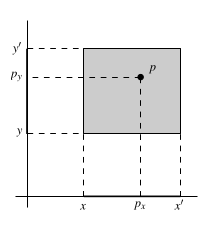
\includegraphics{images/search_range.png}
    \end{center}
    \citetitle{comp-geo}
\end{figure}

\subsection{Construção da Árvore 2-dimensional}
Na construção de uma árvore para 2 dimensões, cada ponto tem uma forma: 
    \[p = (x, y) \]
Escolhemos um eixo para iniciar a construção da árvore. Ordenamos os pontos de $P$ pelo eixo escolhido.
O valor da mediana dos pontos ordenados pelo eixo será o valor de corte do conjunto $P$, e serão criados dois subconjuntos.
Chama-se recursivamente a construção da árvore alternando o eixo e passando os subconjuntos.

\begin{figure}[htb]
    \caption{\label{fig:Fig_3} Árvore 2D}
    \begin{center}
        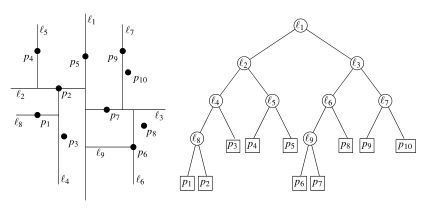
\includegraphics{images/kd_tree1.png}
    \end{center}
\end{figure}


Seja $P$ conjunto de pontos. Inicialmente escolhemos o $eixo-x$. Acompanharemos a troca de eixos segundo a profundidade da árvore.
Caso a profundidade seja $par$, ordenaremos pelo eixo $x$, do contrário pelo eixo $y$.
Fazemos uma $x-ordenação$ em $P$ e encontramos o valor $x_{mediana}$.
Criamos dois subconjuntos $P_1$ e $P_2$ tal que:
    \[P_1 \leftarrow p \forall p_{x} \leq x_{mediana} \]
    \[P_2 \leftarrow p \forall p_{x} > x_{mediana} \]
Agora, recursivamente, repete-se para os dois novos conjuntos criados até restar somente um ponto. Este, por sua vez, será um nó folha.

\begin{algorithm}
    \caption{O algorítimo \Call{ConstroiArvore2D}{$P$, $profundidade=0$}, recebe um conjunto de pontos $P$ no plano e uma profundidade da árvore.
    O algoritmo retorna a raiz de uma árvore 2D}
    \begin{algorithmic}[1]
        \Function{ConstroiArvore2D}{$P$, $profundidade$}
            \If{P contem apenas um ponto}
            \Return $nó \leftarrow ponto$
        \Else
            \If{$profundidade$ é par}
            \State
                Divide P em dois subconjuntos com um linha vertical $l$ pela mediana da $x-coordenada$
                dos pontos em P. Seja $P_1$ o conjunto dos pontos à esquerda de $l$ e seja
                $P_2$ o conjunto de pontos à direita de $l$.
            \Else
            \State
                Divide P em dois subconjuntos com um linha horizontal $l$ pela mediana da $y-coordenada$
                dos pontos em P. Seja $P_1$ o conjunto dos pontos acima de $l$ e seja
                $P_2$ o conjunto de pontos à abaixo de $l$.
            \EndIf
        \EndIf
        \State $v_{esquerda} \leftarrow $ \Call{ConstroiArvore2D}{$P_1, profundidade+1$}
        \State $v_{direita} \leftarrow $ \Call{ConstroiArvore2D}{$P_2, profundidade+1$}
        \State Cria um nó $v$, associamos o valor $l$ e associamos os filhos $v_{esquerda}$ e $v_{direita}$ 

        \Return $v$
        \EndFunction
    \end{algorithmic}
\end{algorithm}

\subsection{Consulta}

Agora retomamos para o algoritmo de consulta. Podemos supor que os pontos na subárvore à esquerda
da raiz, possuindo $x$-coordenada no máximo igual ao valor de $l_1$ armazenado na raiz.
Enquanto os pontos na subárvore à direita do nó raiz possuem $y$-coordenada maior que $l_1$.

A exemplo: a região correspondente do nó \(l_4\) é limitada à esquerda de
\(l_1\) e abaixo de \(y\) do nodo \(l_2\).


\begin{figure}[htb]
    \caption{\label{fig:Fig_4} Área respectiva do nó $l_4$}
    \begin{center}
        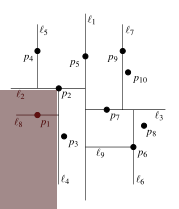
\includegraphics{images/kd_tree2.png}
    \end{center}
\end{figure}

Denotaremos esta área de um nó \(v\) como \(regiao(v)\). A região da raiz é simplesmente
(no caso de uma árvore 2D) o plano inteiro.
Portanto, o algoritmo buscará a subárvore de \(v\) somente se o retângulo de busca intersectar
a \(regiao(v)\).

O algoritmo de busca funciona descendo a árvore, mas visitando somente os nós que a
\(regiao(v)\) intersecta o retângulo da consulta. Quando uma \(regiao(v)\) está contido no
retângulo de busca retornamos todos os pontos na subárvore.
Quando chegarmos nos nós folha temos de checar se o nodo esta dentro da consulta, se estiver,
retorna-o.

Segue o algoritmo que recebe como parâmetros a raiz da arvore2D e o retângulo de consulta \(R\).
Usamos uma chamada \(RetornaSubarvore(v)\) que atravessa a árvore do nó \(v\) e retorna
todos os pontos nas suas folhas. Segue como notação \(filho_{esquerda}(v)\) sendo o filho da esquerda e
\(filho_{direita}(v)\) o filho da direita do nodo \(v\).


\begin{algorithm}
    \caption{A função \Call{BuscaEmArvore2D}{$v$, $consulta$} recebe como parâmetro um nó e uma consulta. E retorna todos os pontos
     dentro da consulta.}
    \begin{algorithmic}[1]
    \Function{BuscaEmArvore}{$v$, $consulta$}
        \If{v é folha}
        \Return  $v$ se estiver dentro da $consulta$
        \Else
            \If{$regiao(filho_{esquerda}(v))$ está contido na $consulta$}
            \State \Return $SubArvore( filho_{esquerda}(v) )$
            \Else
                \If{$regiao(filho_{esquerda}(v))$ intersecta $consulta$}
                \State \Call{BuscaEmArvore2D}{$filho_{esquerda}(v)$, $consulta$}
                \EndIf
            \EndIf
            \If{$regiao(filho_{direita}(v))$ está contido na $consulta$}
            \State \Return $SubArvore(filho_{direita}(v))$
            \Else
                \If{$regiao(filho_{direita}(v))$ intersecta $busca$}
                \State \Call{BuscaEmArvore2D}{$filho_{direita}(v)$, $consulta$}
                \EndIf
            \EndIf
        \EndIf
    \EndFunction
    \end{algorithmic}
\end{algorithm}

A comparação realizada é checar se a área \(consulta\) intersecta a região
de um nodo \(v\). Para isso precisamos computar \(regiao(v)\) para todos os nodos \(v\)
durante a fase de construção da árvore.
Uma alternativa é manter a região salva nas chamadas recursivas usando as linhas guardadas
nos nodos internos. Por exemplo, a região correspondente ao filho esquerda de um nodo
\(v\) em uma profundidade par (no exemplo 2D, analisamos no eixo \(x\)) pode ser calculado com:
\[
    regiao(filho_{esquerda}(v)) = regiao(v) \cap l(v)^{esquerda}
\]
onde \(l(v)\) é a linha que divide o eixo salvo em \(v\), e \(l(v)^{esquerda}\) é a metade
esquerda do plano.
Salvando apenas os intervalos respectivos de cada nível da árvore. 

\section{Resultados}
\begin{figure}[htb]
    \caption{\label{fig:Fig_5} — Resultados de busca com Arvore2D}
    \begin{center}
        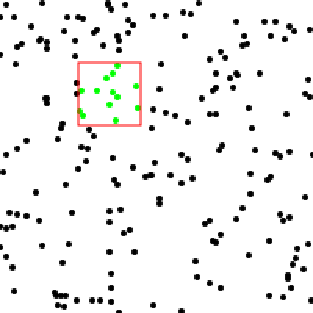
\includegraphics{images/points.pdf}
    \end{center}
\end{figure}


Na Figura 5 temos os pontos:

(70.0, 73.0), (-10.0, 24.0), (0.0, 0.0), (-44.0, 39.0), (-49.0, 3.0), (15.0, 56.0), 
(-9.0, -44.0), (23.0, 21.0), (-43.0, -13.0), (-6.0, -13.0), (18.0, 31.0), (8.0, -19.0),
 (24.0, 13.0)

E a consulta (o retângulo em vermelho) as coordenadas: (-50, -10), (50, 40), (-50, 40), (50, -10)

Retornando corretamente o conjunto de pontos:

(-49.0, 3.0),
(-44.0, 39.0),
(-10.0, 24.0),
(0.0, 0.0),
(18.0, 31.0),
(23.0, 21.0),
(24.0, 13.0)

Sendo facilmente verificável apenas constatando que os valores $x$:
\[ x \leq 50 \textrm{ e } x > -50 \]
\[ y \leq 10 \textrm{ e } y > -10 \]

\section{Arvore de Intervalos}
% ----------------------------------------------------------

% No que diz respeito à estrutura do trabalho, recomenda-se que:
% \begin{alineas}
% 	\item o texto deve ser justificado, digitado em cor preta, podendo utilizar outras cores somente para as ilustrações;
% 	\item utilizar papel branco ou reciclado para impressão;
% 	\item os elementos pré-textuais devem iniciar no anverso da folha, com exceção da ficha catalográfica ou ficha de identificação da obra;
% 	\item os elementos textuais e pós-textuais devem ser digitados no anverso e verso das folhas, quando o trabalho for impresso. As seções primárias devem começar sempre em páginas ímpares, quando o trabalho for impresso. Deixar um espaço entre o título da seção/subseção e o texto e entre o texto e o título da subseção.
% \end{alineas}

% No \autoref{qua:Quadro_1} estão as especificações para a formatação do texto.

% \begin{quadro}[htb]
% 	\centering
% 	\caption{\label{qua:Quadro_1}Formatação do texto.}
% 	\begin{tabular}{|l|p{11cm}|}
% 		\hline
% 		\textbf{Formato do papel} & A4.                                                                                                                                                                                                                                                                                                                                                                                                                                 \\ \hline
% 		\textbf{Impressão}        & A norma recomenda que caso seja necessário imprimir, deve-se utilizar a frente e o verso da página.                                                                                                                                                                                                                                                                                                                                 \\ \hline
% 		\textbf{Margens}          & Superior: 3, Inferior: 2, Interna: 3 e Externa: 2. Usar margens espelhadas quando o  trabalho for impresso.                                                                                                                                                                                                                                                                                                                         \\ \hline
% 		\textbf{Paginação}        & As páginas dos elementos pré-textuais devem ser contadas, mas não numeradas. Para trabalhos digitados somente no anverso, a numeração das páginas deve constar no canto superior direito da página, a 2 cm da borda, figurando a partir da primeira folha da  parte textual. Para trabalhos digitados no anverso e no verso, a numeração deve constar no canto superior direito, no anverso, e no canto superior esquerdo no verso. \\ \hline
% 		\textbf{Espaçamento}      & O texto deve ser redigido com espaçamento entre linhas 1,5, excetuando-se as citações de mais de três linhas, notas de rodapé, referências, legendas das ilustrações e das tabelas, natureza (tipo do trabalho, objetivo, nome da instituição a que é submetido e área de concentração), que devem ser digitados em espaço simples, com fonte menor. As referências devem ser separadas entre si por um espaço simples em branco.   \\ \hline
% 		\textbf{Paginação}        & A contagem inicia na folha de rosto, mas se insere o número da página na introdução até o final do trabalho.                                                                                                                                                                                                                                                                                                                        \\ \hline
% 		\textbf{Fontes sugeridas} & Arial ou Times New Roman.                                                                                                                                                                                                                                                                                                                                                                                                           \\ \hline
% 		\textbf{Tamanho da fonte} & \textbf{Fonte tamanho 12 para o texto}, incluindo os títulos das seções e subseções. As citações com mais de três linhas, notas de rodapé, paginação, dados internacionais de catalogação, legendas e fontes das ilustrações e das tabelas devem ser de tamanho menor. Adotamos, neste \textit{template} \textbf{fonte tamanho 10}.                                                                                                 \\ \hline
% 		\textbf{Nota de rodapé}   & Devem ser digitadas dentro da margem, ficando separadas por um espaço simples por entre as linhas e por filete de 5 cm a partir da margem esquerda. A partir da segunda linha, devem ser alinhadas embaixo da primeira letra da primeira palavra da primeira linha.                                                                                                                                                                 \\ \hline
% 	\end{tabular}
% 	\fonte{\textcite{NBR14724:2011}.}
% \end{quadro}

% % ----------------------------------------------------------
% \subsubsection{As ilustrações}
% % ----------------------------------------------------------

% Independentemente do tipo de ilustração (quadro, desenho, figura, fotografia, mapa, entre outros), a sua identificação aparece na parte superior, precedida da palavra designativa.

% \begin{citacao}
% 	Após a ilustração, na parte inferior, indicar a fonte consultada (elemento obrigatório, mesmo que seja produção do próprio autor), legenda, notas e outras informações necessárias à sua compreensão (se houver). A ilustração deve ser citada no texto e inserida o mais próximo possível do texto a que se refere. \cite[p. 11]{NBR14724:2011}.
% \end{citacao}

% % ----------------------------------------------------------
% \subsubsection{Equações e fórmulas}
% % ----------------------------------------------------------

% As equações e fórmulas devem ser destacadas no texto para facilitar a leitura.  Para numerá-las, usar algarismos arábicos entre parênteses e alinhados à direita. Pode-se adotar uma entrelinha maior do que a usada no texto \cite{NBR14724:2011}.

% Exemplos, \autoref{eq:Eq_1} e \autoref{eq:Eq_2}.

% \begin{equation}\label{eq:Eq_1}
% 	\gls{C} = 2 \gls{pi} \gls{r}
% \end{equation}

% \begin{equation}\label{eq:Eq_2}
% 	\gls{A} = \gls{pi} \gls{r}^2
% \end{equation}
% ----------------------------------------------------------
\section{Arvore de Segmentos}
% ----------------------------------------------------------

% De acordo com \textcite{ibge1993}, tabela é uma forma não discursiva de apresentar informações em que os números representam a informação central. Ver \autoref{tab:Tab_1}.

% \begin{table}[htb]
% 	\ABNTEXfontereduzida
% 	\caption{\label{tab:Tab_1}Médias concentrações urbanas 2010-2011.}
% 	\begin{tabular}{@{}p{3.0cm}p{1.5cm}p{2cm}p{2.5cm}p{2.5cm}p{2.5cm}@{}}
% 		\toprule
% 		\textbf{Média concentração urbana} & \multicolumn{2}{l}{\textbf{População}} & \textbf{Produto Interno Bruto – PIB (bilhões R\$)} & \textbf{Número de empresas} & \textbf{Número de unidades locais}         \\ \midrule
% 		\textbf{Nome}                      & \textbf{Total}                         & \textbf{No Brasil}                                 &                             &                                    &       \\
% 		Ji-Paraná (RO)                     & 116 610                                & 116 610                                            & 1,686                       & 2 734                              & 3 082 \\
% 		Parintins (AM)                     & 102 033                                & 102 033                                            & 0,675                       & 634                                & 683   \\
% 		Boa Vista (RR)                     & 298 215                                & 298 215                                            & 4,823                       & 4 852                              & 5 187 \\
% 		Bragança (PA)                      & 113 227                                & 113 227                                            & 0,452                       & 654                                & 686   \\ \bottomrule
% 	\end{tabular}
% 	\fonte{\textcite{ibge2016}.}
% \end{table}